\newpage
\section{Progettazione}
\subsection{Studio dell'utenza finale}
\subsubsection{Utente generico}
L'utenza maggiore che ci si aspetta potrà visitare questo sito è composta principalmente da persone dal profilo informatico medio basso alla ricerca di informazioni dettagliate riguardo la fornitura dell'azienda, probabilmente in mobilità. L'applicativo web offre informazioni relative ad un'azienda agricola, posto che in genere non è frequentato pubblicamente per svago. Per questo motivo la maggior parte delle informazioni sono contenute in pagine statiche. Inoltre si sono create le pagine di \textbf{servizi} e \textbf{prodotti} che, pur non permettendo un acquisto o una prenotazione on line, offrono all'utente la possibilità di vedere le offerte e di contattare l'azienda telefonicamente nella scheda \textbf{contattaci}.
\subsubsection{Azienda business-to-business}
Ci si può aspettare inoltre che qualche azienda in cerca di un commercio business-to-business di grano visiti il sito. In questo caso le pagine statiche di \textbf{home} e \textbf{chi siamo} offrono una panoramica sulla storia e sulla solidità dell'azienda, pubblicizzandola. Ci si aspetta quindi un utente più esperto nell'utilizzo di un PC o smartphone, che quindi potrà eventualmente anche creare un messaggio con più informazioni, in attesa di un contatto telematico, sfruttando il form preparato nella scheda \textbf{contattaci}.
\subsubsection{Amministratore}
Il sito potrà essere gestito da uno o più amministratori ingaggiati dall'azienda, che si supporranno essere persone mediamente più esperte nell'utilizzo di un computer, che si occuperanno di amminsitrare il sito da una postazione principalmente fissa.

\subsection{Struttura}
\subsubsection{Utente generico}
\paragraph{Barra di navigazione}
~\\Il sito è stato pensato per avere una navigazione a barra orizzontale fissa posta in alto sullo schermo. Le pagine del sito sono, per quanto riguarda gli utenti non registrati:
\begin{itemize}
	\item \textbf{Home}
	\item \textbf{Chi siamo}
	\item \textbf{Prodotti}
	\item \textbf{Servizi}
	\item \textbf{Contattaci}
\end{itemize}
Nella barra è presente il logo dell'azienda e i pulsanti che portano alle altre pagine del sito. In particolare, il pulsante indicante la pagina attuale è incorniciato, mentre gli altri, se il mouse ci passa sopra, vengono sottolineati. All'interno della barra, posto subito sotto, è presente il breadcrumb: a sinistra si occupa di indicare la posizione attuale all'interno del sito, a destra è presente un'ancora che porta direttamente al contenuto. Se si utilizza il \emph{tab} da tastiera si potrà apprezzare che questo è il primo link cliccabile. Nell'immagine seguente è possibile vedere un esempio della barra:
\begin{figure}[h!]
	\centerline{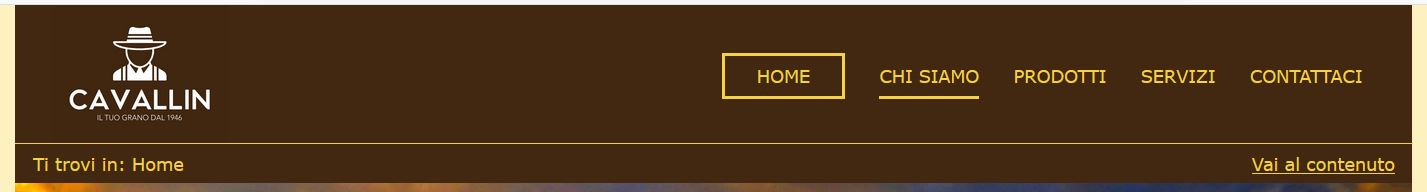
\includegraphics[scale=0.45]{img/barra_navigazione.jpg}}
	\caption{Barra di navigazione per l'utente generico}
	\label{fig:navbarGU}
\end{figure}
~\\Sebbene non facente parte della barra, è presente un'àncora fissata in basso a destra sul sito che si occupa di riportare il lettore all'inizio del contenuto.
\begin{figure}[h!]
	\centerline{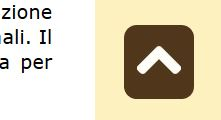
\includegraphics[scale=0.45]{img/jump_to_menu.jpg}}
	\caption{Ancora all'inizio del contenuto}
	\label{fig:anchor}
\end{figure}
\paragraph{Corpo}
~\\Il corpo è disposto con layout orizzontale all'interno della pagina, con una larghezza massima fissata, in modo da renderlo più elegante anche con risoluzioni elevate. La maggior parte dei contenuti è organizzata in rettangoli, ognuno dei quali contiene il titolo della sotto sezione, il testo e un'immagine indicativa.
Nell'immagine subito successiva si può notare un esempio:
\begin{figure}[h!]
	\centerline{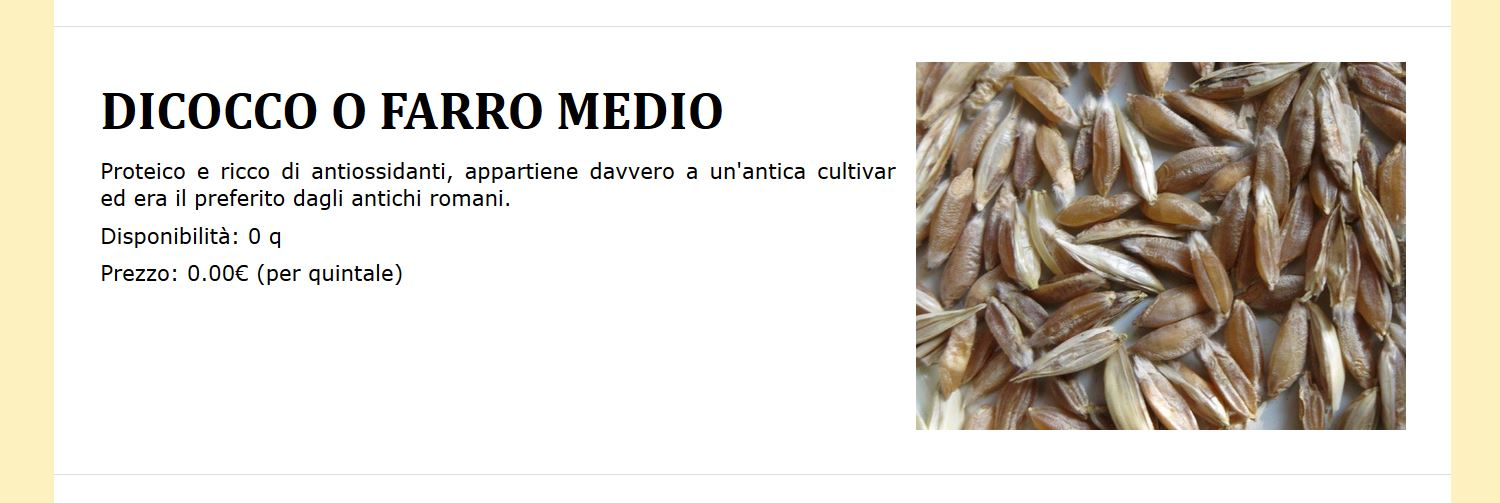
\includegraphics[scale=0.40]{img/corpo_esempio.jpg}}
	\caption{Esempio di sezione del corpo}
	\label{fig:corpoGU}
\end{figure}
\paragraph{Pié di pagina}
~\\A pié di pagina si possono trovare delle informazioni relative al progetto, ovvero il nome dei partecipanti alla creazione del sito e le certificazioni di adesione agli standard \emph{XHTML} e \emph{CSS3}. Inoltre è presente un collegamento alla sezione di amministrazione, alla quale si può accede solo se già registrati da un altro amministratore.
\begin{figure}[h!]
	\centerline{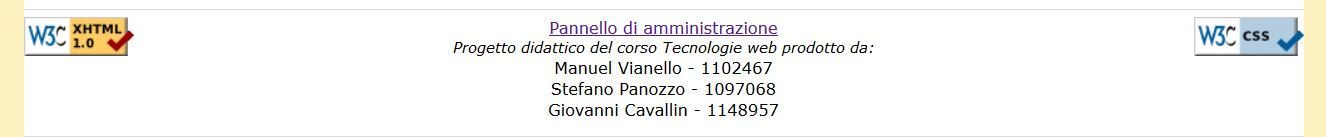
\includegraphics[scale=0.45]{img/footer.jpg}}
	\caption{Pié di pagina del sito}
	\label{fig:footer}
\end{figure}
\subsubsection{Amministratore}
La GUI si differenzia da quella dell'utente base per alcune particolarità.
\paragraph{Barra di navigazione}
~\\Sono presenti altre pagine in cui navigare:
\begin{itemize}
	\item \textbf{Pannello amministrazione}
	\item \textbf{Prodotti}
	\item \textbf{Servizi}
	\item \textbf{Storico prenotazioni}
	\item \textbf{Prenotazioni}
	\item \textbf{Clienti}
	\item \textbf{Amministratori}
\end{itemize}
Nel breadcrumb poi, al posto del \emph{Vai al contenuto}, sono presenti due link: un \emph{Torna al sito} e un pulsante di \emph{Logout}, che hanno lo stesso risultato di riportare l'utente al sito generico, ma che nel secondo caso chiude la sessione di amministratore. Viene infine rimossa l'àncora per tornare all'inizio della pagina.
\begin{figure}[h!]
	\centerline{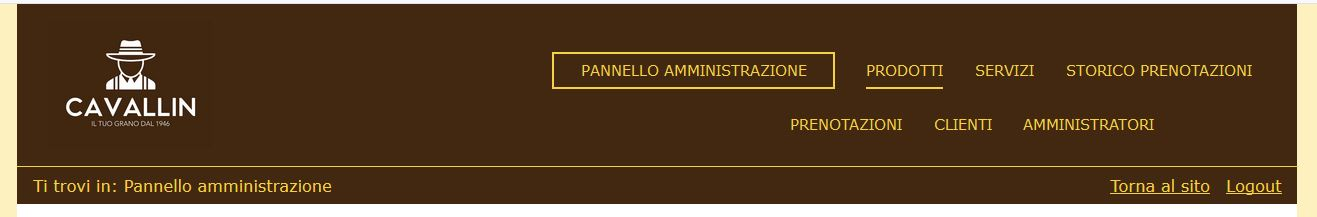
\includegraphics[scale=0.49]{img/barra_navigazione_admin.jpg}}
	\caption{Barra di navigazione per l'amministratore}
	\label{fig:navbarAD}
\end{figure}
\paragraph{Corpo}
~\\La struttura rimane pressoché invariata, ma in ognuna di esse - meno la \textbf{Storico prenotazioni} - è presente a fondo pagina un modulo di aggiunta informazioni.
\begin{figure}[h!]
	\centerline{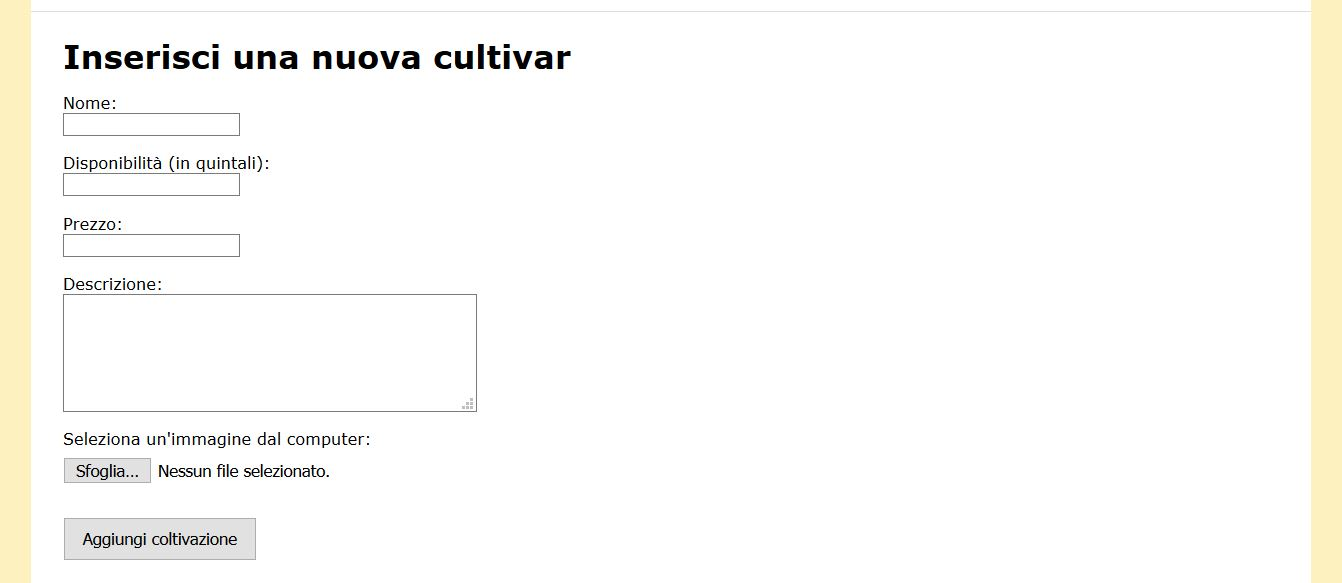
\includegraphics[scale=0.49]{img/add_form.jpg}}
	\caption{Form di aggiunta informazioni}
	\label{fig:addForm}
\end{figure}
\paragraph{Pié di pagina}
~\\Nel pié di pagina invece viene solamente rimosso il link al pannello di amministrazione poiché inutile.










